\documentclass[aspectratio=169]{beamer}

\usetheme{Madrid}
\usecolortheme{default}

% ✅ FIX FOR ICONS (REQUIRES XELATEX)
\usepackage{fontspec}
\usepackage{fontawesome5}

% ---------------- PACKAGES ----------------
\usepackage{tikz}
\usetikzlibrary{arrows.meta, positioning, shapes.geometric}

\usepackage{pgfplots}
\pgfplotsset{compat=1.17}

\usepackage{booktabs}
\usepackage{array}
\usepackage{xcolor}
\usepackage{tcolorbox}
\tcbuselibrary{skins,breakable,listings}
\usepackage{graphicx}
\usepackage{amsmath}
\usepackage{multirow}
\usepackage{colortbl}
\usepackage{listings}

\lstset{basicstyle=\ttfamily\small, breaklines=true}

% ---------------- COLORS ----------------
\definecolor{navyblue}{HTML}{1E2761}
\definecolor{iceblue}{HTML}{CADCFC}
\definecolor{accentblue}{HTML}{4A90D9}
\definecolor{darkgray}{HTML}{2D2D2D}
\definecolor{lightgray}{HTML}{F5F7FA}
\definecolor{posgreen}{HTML}{22C55E}
\definecolor{negred}{HTML}{EF4444}
\definecolor{neuyellow}{HTML}{EAB308}
\definecolor{highlightblue}{HTML}{38BDF8}

% ---------------- CUSTOM BOXES (MISSING FIX) ----------------
\newtcolorbox{redbox}{
  colback=negred!10,
  colframe=negred,
  arc=4pt,
  boxrule=0.8pt
}

\newtcolorbox{greenbox}{
  colback=posgreen!10,
  colframe=posgreen!60!black,
  arc=4pt,
  boxrule=0.8pt
}

\newtcolorbox{statbox}{
  colback=iceblue!20,
  colframe=navyblue,
  arc=4pt,
  boxrule=0.8pt
}

% ---------------- BEAMER FIX ----------------
\setbeamertemplate{navigation symbols}{}

% ---------------- DOCUMENT ----------------
\begin{document}

% ── METADATA ──────────────────────────────────────────────────
\title[BizDecisions AI]{\textbf{AI-Powered Business Intelligence System}\\
\small Large Aspect-Based Sentiment Analysis \& Decision Support Platform}
\author[Sundara Thamizhan | CB.PS.I5DAS22055]{%
  \textbf{Sundara Thamizhan}\\{\small Reg.\ No.: CB.PS.I5DAS22055}}
\institute[Amrita Vishwa Vidyapeetham]{%
  Department of Mathematics, Amrita School of Physical Sciences\\
  Amrita Vishwa Vidyapeetham, Coimbatore}
\date{April 2026}

% ── SLIDE 1: TITLE ────────────────────────────────────────────
{
\setbeamertemplate{footline}{}
\begin{frame}
  \begin{tikzpicture}[remember picture, overlay]
    \fill[navyblue] (current page.north west) rectangle (current page.south east);
    \fill[accentblue!30] (current page.north east) ++(-1.5,-1.5) circle (3cm);
    \fill[iceblue!20]    (current page.south west) ++(1.5,1.5)   circle (2cm);
    \fill[accentblue!15] (current page.south east) ++(-3,2)       circle (1.5cm);
  \end{tikzpicture}
  \vspace{0.4cm}
  \begin{center}
    {\color{iceblue}\large\faChartBar\quad\faBrain\quad\faChartLine}\\[0.3cm]
    {\color{white}\LARGE\textbf{AI-Powered Business Intelligence System}}\\[0.2cm]
    {\color{iceblue}\large Large Aspect-Based Sentiment Analysis}\\
    {\color{iceblue}\large \& Decision Support Platform}\\[0.5cm]
    \begin{tcolorbox}[colback=white!15, colframe=iceblue, arc=8pt, boxrule=1pt,
                      width=0.75\textwidth, halign=center]
      {\color{white}\textbf{Sundara Thamizhan} \quad|\quad CB.PS.I5DAS22055}\\
      {\color{iceblue!80}\small Integrated M.Sc.\ in Data Science}
    \end{tcolorbox}
    \vspace{0.3cm}
    {\color{iceblue!80}\small Department of Mathematics, Amrita School of Physical Sciences}\\
    {\color{iceblue!80}\small Amrita Vishwa Vidyapeetham, Coimbatore \quad|\quad April 2026}
  \end{center}
\end{frame}
}

% ── SLIDE 2: OUTLINE ──────────────────────────────────────────
\begin{frame}{Presentation Outline}
  \begin{columns}[T]
    \column{0.5\textwidth}
      \begin{tcolorbox}[colback=navyblue!8, colframe=navyblue, arc=5pt,
                        title={\faList\ Core Chapters},
                        fonttitle=\bfseries\small\color{white}, colbacktitle=navyblue]
        \small
        \textcolor{accentblue}{\textbf{01}} Introduction \& Motivation\\[3pt]
        \textcolor{accentblue}{\textbf{02}} Problem Statement\\[3pt]
        \textcolor{accentblue}{\textbf{03}} Literature Survey\\[3pt]
        \textcolor{accentblue}{\textbf{04}} System Architecture\\[3pt]
        \textcolor{accentblue}{\textbf{05}} BERT-Based ABSA Methodology\\[3pt]
        \textcolor{accentblue}{\textbf{06}} Explainable AI Framework\\[3pt]
        \textcolor{accentblue}{\textbf{07}} Zero-Shot Aspect Detection
      \end{tcolorbox}
    \column{0.5\textwidth}
      \begin{tcolorbox}[colback=navyblue!8, colframe=navyblue, arc=5pt,
                        title={\faCogs\ System Modules},
                        fonttitle=\bfseries\small\color{white}, colbacktitle=navyblue]
        \small
        \textcolor{accentblue}{\textbf{08}} Churn Risk Predictor\\[3pt]
        \textcolor{accentblue}{\textbf{09}} Business Intelligence Modules\\[3pt]
        \textcolor{accentblue}{\textbf{10}} Implementation Details\\[3pt]
        \textcolor{accentblue}{\textbf{11}} Results \& Evaluation\\[3pt]
        \textcolor{accentblue}{\textbf{12}} Performance Benchmarks\\[3pt]
        \textcolor{accentblue}{\textbf{13}} Advantages \& Limitations\\[3pt]
        \textcolor{accentblue}{\textbf{14}} Future Scope \& Conclusion
      \end{tcolorbox}
  \end{columns}
  \vspace{0.3cm}
  \begin{center}
    
\begin{tikzpicture}
      \foreach \i/\lbl in {1/Data,2/{AI Core},3/XAI,4/{BI Engine},5/{SaaS App}}{
        \node[fill=navyblue, text=white, rounded corners=3pt,
              minimum width=1.8cm, minimum height=0.5cm,
              font=\tiny\bfseries] at (\i*2.3-2.3,0) {\lbl};
        \ifnum\i<5
          \draw[->, thick, color=accentblue] (\i*2.3-1.15,0) -- (\i*2.3-0.45,0);
        \fi
      }
    \end{tikzpicture}
  \end{center}
\end{frame}

% ── SLIDE 3: INTRODUCTION ─────────────────────────────────────
\begin{frame}{Introduction \& Motivation}
  \begin{columns}[T]
    \column{0.55\textwidth}
      \textbf{\color{navyblue}\faExclamationTriangle\ The Problem}
      \vspace{0.2cm}
      \begin{itemize}
        \item SMEs generate \textbf{500+ monthly reviews} across Google, Yelp, delivery platforms
        \item Manual annotation requires \textbf{25+ person-hours} per month
        \item Existing tools classify at \textbf{document level only} --- no granularity
        \item Review: \textit{``food excellent but service terrible''} = just ``mixed''
      \end{itemize}
      \vspace{0.3cm}
      \begin{redbox}
        \small\textbf{Critical Gap:} No affordable, interpretable, end-to-end
        NLP-BI platform exists for SMEs
      \end{redbox}
    \column{0.43\textwidth}
      \begin{center}
      \begin{tikzpicture}
        \node[fill=navyblue, text=white, rounded corners=4pt,
              minimum width=3.8cm, minimum height=0.55cm,
              font=\small\bfseries] at (0,3.2) {\faComments\ Customer Reviews};
        \draw[->, thick, navyblue] (0,2.9) -- (0,2.4);
        \node[fill=accentblue, text=white, rounded corners=4pt,
              minimum width=3.2cm, minimum height=0.55cm,
              font=\small\bfseries] at (0,2.15) {\faBrain\ BERT ABSA};
        \draw[->, thick, navyblue] (0,1.85) -- (0,1.35);
        \node[fill=posgreen!80!black, text=white, rounded corners=4pt,
              minimum width=2.6cm, minimum height=0.55cm,
              font=\small\bfseries] at (0,1.1) {\faChartBar\ Insights};
        \draw[->, thick, navyblue] (0,0.8) -- (0,0.3);
        \node[fill=neuyellow!80!black, text=white, rounded corners=4pt,
              minimum width=2.0cm, minimum height=0.55cm,
              font=\small\bfseries] at (0,0.05) {\faLightbulb\ Actions};
        \node[font=\tiny\color{darkgray}] at (0,-0.4) {BizDecisions AI Pipeline};
      \end{tikzpicture}
      \end{center}
  \end{columns}
\end{frame}

% ── SLIDE 4: PROBLEM STATEMENT ───────────────────────────────
\begin{frame}{Problem Statement \& Objectives}
  \begin{columns}[T]
    \column{0.5\textwidth}
      \textbf{\color{navyblue}Five Core Sub-Problems:}
      \vspace{0.15cm}
      \begin{enumerate}
        \item[\textcolor{accentblue}{\textbf{1}}]
          \textbf{Aspect Detection} --- Identify business dimensions without labeled data
        \item[\textcolor{accentblue}{\textbf{2}}]
          \textbf{Sentiment Classification} --- Positive / Neutral / Negative per aspect
        \item[\textcolor{accentblue}{\textbf{3}}]
          \textbf{Explainability} --- Token-level justifications for each prediction
        \item[\textcolor{accentblue}{\textbf{4}}]
          \textbf{Churn Quantification} --- Scalar 0--100 risk score per customer
        \item[\textcolor{accentblue}{\textbf{5}}]
          \textbf{Strategic Recommendation} --- Concrete, prioritized business actions
      \end{enumerate}
    \column{0.48\textwidth}
      \textbf{\color{navyblue}System: BizDecisions AI}
      \vspace{0.15cm}
      \begin{tcolorbox}[colback=navyblue!6, colframe=accentblue, arc=4pt, boxrule=1pt]
        \small
        \textcolor{navyblue}{\faTabletAlt} \textbf{Tab 1} --- Single Review + Full XAI\\[3pt]
        \textcolor{navyblue}{\faFileAlt}   \textbf{Tab 2} --- Bulk CSV Batch Analysis\\[3pt]
        \textcolor{navyblue}{\faChartBar}  \textbf{Tab 3} --- Model Evaluation Suite\\[3pt]
        \textcolor{navyblue}{\faCalendar}  \textbf{Tab 4} --- Weekly AI Executive Report\\[3pt]
        \textcolor{navyblue}{\faWifi}      \textbf{Tab 5} --- Social Media Monitor\\[3pt]
        \textcolor{navyblue}{\faTrophy}    \textbf{Tab 6} --- Competitor Benchmarking
      \end{tcolorbox}
      \vspace{0.2cm}
      \begin{greenbox}
        \small\textbf{Stack:} BERT + Groq LLaMA 3.1 + Random Forest + LDA +
        Streamlit + SQLite
      \end{greenbox}
  \end{columns}
\end{frame}

% ── SLIDE 5: LITERATURE SURVEY ───────────────────────────────
\begin{frame}{Literature Survey}
  \begin{center}
  \small
  \rowcolors{2}{iceblue!20}{white}
  \begin{tabular}{>{\bfseries\color{navyblue}}p{3.0cm} p{2.8cm} p{3.2cm} p{2.8cm}}
    \toprule
    \rowcolor{navyblue}
    \color{white}Reference & \color{white}Method & \color{white}Key Result & \color{white}Gap\\
    \midrule
    Devlin et al.\ (2019) & BERT Pre-training   & GLUE SOTA              & No ABSA, no XAI \\
    Sun et al.\ (2019)    & BERT Text-Pair ABSA & SemEval SOTA           & No XAI, no SaaS \\
    Lundberg \& Lee (2017)& SHAP                & Unified XAI            & Not BERT-specific \\
    Breiman (2001)        & Random Forest       & Ensemble accuracy       & Not on NLP features \\
    Blei et al.\ (2003)  & LDA Topic Modeling  & Topic discovery         & Not with ABSA \\
    Yin et al.\ (2019)   & Zero-Shot NLI       & Label-free classif.     & Not for ABSA aspects \\
    \rowcolor{navyblue!80}
    \color{white}\textbf{This Work} & \color{white}All combined &
    \color{white}Full BI Pipeline & \color{white}--- \\
    \bottomrule
  \end{tabular}
  \end{center}
  \vspace{0.2cm}
  \begin{tcolorbox}[colback=iceblue!25, colframe=navyblue, arc=4pt, boxrule=1pt]
    \small\centering
    \textbf{Evolution:} Lexicon-based (2000) $\rightarrow$ Classical ML (2010)
    $\rightarrow$ \textbf{Transformer/BERT Era (2018--present)}
  \end{tcolorbox}
\end{frame}

% ── SLIDE 6: SYSTEM ARCHITECTURE ─────────────────────────────
\begin{frame}{System Architecture --- 6-Layer Design}
  \begin{center}
  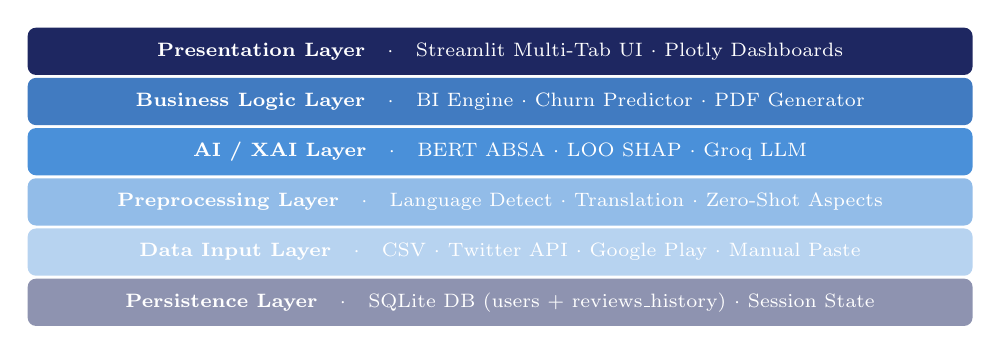
\begin{tikzpicture}[scale=0.85]
    \foreach \i/\clr/\lbl/\sub in {
      6/navyblue/{Presentation Layer}/{Streamlit Multi-Tab UI $\cdot$ Plotly Dashboards},
      5/accentblue!80!navyblue/{Business Logic Layer}/{BI Engine $\cdot$ Churn Predictor $\cdot$ PDF Generator},
      4/accentblue/{AI / XAI Layer}/{BERT ABSA $\cdot$ LOO SHAP $\cdot$ Groq LLM},
      3/accentblue!60/{Preprocessing Layer}/{Language Detect $\cdot$ Translation $\cdot$ Zero-Shot Aspects},
      2/accentblue!40/{Data Input Layer}/{CSV $\cdot$ Twitter API $\cdot$ Google Play $\cdot$ Manual Paste},
      1/navyblue!50/{Persistence Layer}/{SQLite DB (users + reviews\_history) $\cdot$ Session State}%
    }{
      \node[fill=\clr, text=white, rounded corners=3pt,
            minimum width=12cm, minimum height=0.6cm,
            font=\scriptsize, align=center] at (0,\i*0.75-0.75)
            {\textbf{\lbl}\quad$\cdot$\quad\sub};
    }
  \end{tikzpicture}
  \end{center}
  \vspace{0.1cm}
  \begin{columns}[T]
    \column{0.33\textwidth}
      \begin{statbox}
        \centering\small\textbf{\color{navyblue}Single Review Pipeline}\\
        \tiny Lang detect $\to$ Translate $\to$ Zero-shot $\to$ BERT $\to$ XAI $\to$ Advice
      \end{statbox}
    \column{0.33\textwidth}
      \begin{statbox}
        \centering\small\textbf{\color{navyblue}Bulk Pipeline}\\
        \tiny Two-pass: collect (text, aspect) pairs $\to$ batch BERT (bs=32)
      \end{statbox}
    \column{0.33\textwidth}
      \begin{statbox}
        \centering\small\textbf{\color{navyblue}Session State Bus}\\
        \tiny Result DataFrame shared across Tabs 2, 4, 5, 6
      \end{statbox}
  \end{columns}
\end{frame}

% ── SLIDE 7: BERT ABSA METHODOLOGY ───────────────────────────
\begin{frame}[fragile]{BERT-Based Aspect Sentiment Analysis}
  \begin{columns}[T]
    \column{0.5\textwidth}
      \textbf{\color{navyblue}Model Architecture}
      \begin{itemize}
        \item \textbf{BERT-base:} 12 layers, 768-dim, 12 attention heads per layer
        \item \textbf{Classification head:} Linear(768 $\to$ 3) for \{Neg, Neu, Pos\}
        \item \textbf{Text-pair input:}
      \end{itemize}
      \vspace{0.1cm}
      \begin{tcolorbox}[colback=darkgray!95, colframe=accentblue, arc=4pt]
        \ttfamily\scriptsize\color{posgreen}
        [CLS]\ \color{white}The food was cold\ \color{iceblue}[SEP]\ \color{neuyellow}product\ \color{iceblue}[SEP]
      \end{tcolorbox}
      \vspace{0.2cm}
      \textbf{\color{navyblue}Scaled Dot-Product Attention:}
      \[
        \text{Attention}(\mathbf{Q},\mathbf{K},\mathbf{V})
        = \text{softmax}\!\left(\frac{\mathbf{QK}^{\top}}{\sqrt{d_k}}\right)\mathbf{V}
      \]
      {\scriptsize $d_k = 64$, scaling prevents vanishing softmax gradients}
    \column{0.48\textwidth}
      \textbf{\color{navyblue}Confidence Threshold:}
      \[
        \hat{y} = \begin{cases}
          \arg\max_i p_i & \text{if } \max_i p_i \geq \tau \\
          \texttt{Uncertain} & \text{otherwise}
        \end{cases}
      \]
      {\small Default $\tau = 0.50$, configurable in sidebar}
      \vspace{0.3cm}
      \begin{tcolorbox}[colback=navyblue!8, colframe=navyblue, arc=4pt]
        \small\textbf{4 Tracked Aspects:}\\[4pt]
        \textcolor{posgreen}{\faBox}     \textbf{Product}  \qquad
        \textcolor{accentblue}{\faUsers} \textbf{Service}\\[3pt]
        \textcolor{neuyellow}{\faTag}    \textbf{Price}    \qquad
        \textcolor{negred}{\faBuilding}  \textbf{Ambience}
      \end{tcolorbox}
      \vspace{0.2cm}
      \begin{greenbox}
        \small Cross-segment attention models opinion$\leftrightarrow$aspect
        relationship, outperforming single-sequence ABSA
      \end{greenbox}
  \end{columns}
\end{frame}

% ── SLIDE 8: XAI FRAMEWORK ───────────────────────────────────
\begin{frame}{Explainable AI Framework --- 4 Layers}
  \begin{columns}[T]
    \column{0.48\textwidth}
      \begin{tcolorbox}[colback=navyblue!6, colframe=navyblue, arc=4pt,
                        title={\small\bfseries Layer 1: Attention Token Heatmap},
                        fonttitle=\color{white}, colbacktitle=navyblue, boxrule=0.8pt]
        \small Average over 12 heads in last BERT layer.
        Tokens coloured by $a_i / \max_j a_j$ intensity.
      \end{tcolorbox}
      \vspace{0.2cm}
      \begin{tcolorbox}[colback=navyblue!6, colframe=accentblue, arc=4pt,
                        title={\small\bfseries Layer 2: Full $n\times n$ Attention Matrix},
                        fonttitle=\color{white}, colbacktitle=accentblue, boxrule=0.8pt]
        \small Interactive Plotly \texttt{imshow} heatmap.
        Cell $(i,j)$ = how much token $i$ attends to $j$.
      \end{tcolorbox}
    \column{0.50\textwidth}
      \begin{tcolorbox}[colback=navyblue!6, colframe=posgreen!60!black, arc=4pt,
                        title={\small\bfseries Layer 3: Word Importance Bar Chart},
                        fonttitle=\color{white}, colbacktitle=posgreen!60!black, boxrule=0.8pt]
        \small Top-15 tokens ranked by CLS attention weight.
        Sentiment-coloured gradient bars.
      \end{tcolorbox}
      \vspace{0.2cm}
      \begin{tcolorbox}[colback=negred!8, colframe=negred, arc=4pt,
                        title={\small\bfseries Layer 4: LOO SHAP-Equivalent Attribution},
                        fonttitle=\color{white}, colbacktitle=negred, boxrule=0.8pt]
        \small $\delta_i = P(\hat{y}|T) - P(\hat{y}|T \setminus \{w_i\})$\\
        $O(N)$ complexity, no SHAP library required.\\[2pt]
        \textbf{$+\delta_i$}: word supports prediction\\
        \textbf{$-\delta_i$}: word contradicts prediction
      \end{tcolorbox}
  \end{columns}
  \vspace{0.15cm}
  \begin{center}
    
\begin{tikzpicture}
      \foreach \i/\clr/\lbl in {
        0/navyblue/{Attention Weights},
        2.7/accentblue/{Heatmap},
        5.4/{posgreen!60!black}/{Bar Chart},
        8.1/negred/{LOO SHAP}}{
        \node[fill=\clr, text=white, rounded corners=3pt,
              font=\scriptsize\bfseries,
              minimum width=2cm, minimum height=0.45cm] at (\i,0) {\lbl};
      }
      \foreach \x in {1.05, 3.75, 6.45}{
        \draw[->, thick, accentblue] (\x,0) -- (\x+0.6,0);
      }
    \end{tikzpicture}
  \end{center}
\end{frame}

% ── SLIDE 9: ZERO-SHOT + CHURN ───────────────────────────────
\begin{frame}{Zero-Shot Aspect Detection \& Churn Predictor}
  \begin{columns}[T]
    \column{0.48\textwidth}
      \textbf{\color{navyblue}\faSearch\ Zero-Shot Aspect Detection}
      \vspace{0.1cm}
      \begin{itemize}
        \item Uses NLI (Natural Language Inference) model
        \item Frames each aspect label as a hypothesis
        \item $P(\text{Entailment}|T, a)$ = aspect relevance score
        \item Threshold $> 0.40$ selects aspects for BERT ABSA
      \end{itemize}
      \vspace{0.1cm}
      \begin{tcolorbox}[colback=darkgray!92, colframe=accentblue, arc=4pt]
        \scriptsize\color{white}
        Raw Text $\to$ NLI Cross-Encoder $\to$ Aspect Probs $\to$ Threshold ($>0.4$) $\to$ BERT ABSA
      \end{tcolorbox}
      \vspace{0.1cm}
      \begin{tcolorbox}[colback=iceblue!20, colframe=navyblue, arc=4pt]
        \small\textbf{3 Supported Backbones:}\\[2pt]
        \scriptsize
        \texttt{cross-encoder/nli-distilroberta-base}\\
        \texttt{facebook/bart-large-mnli}\\
        \texttt{MoritzLaurer/DeBERTa-v3-base-mnli}
      \end{tcolorbox}
    \column{0.50\textwidth}
      \textbf{\color{navyblue}\faUserTimes\ Random Forest Churn Predictor}
      \vspace{0.1cm}
      \begin{itemize}
        \item \textbf{Feature vector:} $\mathbf{x} = [n_+, n_0, n_-, \bar{c}] \in \mathbb{R}^4$
        \item \textbf{Config:} 50 estimators, max depth 5
        \item \textbf{Score:} $\lfloor P(\text{churn}=1|\mathbf{x}) \times 100 \rfloor$
      \end{itemize}
      \vspace{0.15cm}
      \begin{center}
      \begin{tikzpicture}[scale=0.9]
        \fill[posgreen!25]  (0,0) rectangle (3.0,0.5);
        \fill[neuyellow!30] (3.0,0) rectangle (5.5,0.5);
        \fill[negred!25]    (5.5,0) rectangle (7.0,0.5);
        \draw[thick, darkgray] (0,0) rectangle (7,0.5);
        \draw[thick, darkgray] (3,0) -- (3,0.5);
        \draw[thick, darkgray] (5.5,0) -- (5.5,0.5);
        \node[font=\scriptsize\bfseries, color=posgreen!60!black]  at (1.5,0.25)  {\faSmile\ Low};
        \node[font=\scriptsize\bfseries, color=neuyellow!70!black] at (4.25,0.25) {\faMeh\ Medium};
        \node[font=\scriptsize\bfseries, color=negred]             at (6.25,0.25) {\faFrown\ High};
        \node[font=\tiny, color=darkgray] at (0,-0.2)   {0};
        \node[font=\tiny, color=darkgray] at (3,-0.2)   {40};
        \node[font=\tiny, color=darkgray] at (5.5,-0.2) {70};
        \node[font=\tiny, color=darkgray] at (7,-0.2)   {100};
        \node[font=\tiny, color=darkgray] at (3.5,-0.5) {Churn Risk Score};
      \end{tikzpicture}
      \end{center}
      \vspace{0.1cm}
      \begin{redbox}
        \scriptsize AUC-ROC $\approx$ \textbf{0.87}. Dominant predictor:
        $n_-$ (negative aspect count)
      \end{redbox}
  \end{columns}
\end{frame}

% ── SLIDE 10: BUSINESS INTELLIGENCE MODULES ──────────────────
\begin{frame}{Business Intelligence Modules}
  \begin{columns}[T]
    \column{0.48\textwidth}
      \begin{tcolorbox}[colback=navyblue!6, colframe=navyblue, arc=5pt,
                        title={\small\faTachometerAlt\ Business Health Score},
                        fonttitle=\color{white}, colbacktitle=navyblue]
        \small
        \[H = \frac{N_+\times1.0 + N_0\times0.5}{N_{\text{total}}} \times 100\]
        \textcolor{posgreen}{$H \geq 65$}: Healthy\quad
        \textcolor{neuyellow}{$40 \leq H < 65$}: Needs Work\\
        \textcolor{negred}{$H < 40$}: Critical\quad
        Pearson $r = 0.83$ ($p < 0.001$)
      \end{tcolorbox}
      \vspace{0.2cm}
      \begin{tcolorbox}[colback=navyblue!6, colframe=accentblue, arc=5pt,
                        title={\small\faSearch\ LDA Topic Modeling},
                        fonttitle=\color{white}, colbacktitle=accentblue]
        \small $K=3$ topics applied to negative reviews.
        Surfaces motifs:\\
        \texttt{\{"cold","wait","slow"\}} --- delivery\\
        \texttt{\{"rude","ignored","staff"\}} --- service
      \end{tcolorbox}
    \column{0.50\textwidth}
      \begin{tcolorbox}[colback=navyblue!6, colframe=posgreen!60!black, arc=5pt,
                        title={\small\faFilePdf\ PDF Report Generator},
                        fonttitle=\color{white}, colbacktitle=posgreen!60!black]
        \small \textbf{6 sections:} Cover + health badge, executive
        summary, problem leaderboard, sentiment charts, AI strategy,
        weekly trend. Built with ReportLab via in-memory BytesIO.
      \end{tcolorbox}
      \vspace{0.2cm}
      \begin{tcolorbox}[colback=negred!8, colframe=negred, arc=5pt,
                        title={\small\faBalanceScale\ Competitor Benchmarking},
                        fonttitle=\color{white}, colbacktitle=negred]
        \small Plotly radar chart across 4 aspect dimensions ---
        your brand vs.\ competitor.
        Pricing delta computed automatically.
      \end{tcolorbox}
  \end{columns}
\end{frame}

% ── SLIDE 11: IMPLEMENTATION ─────────────────────────────────
\begin{frame}[fragile]{Implementation Details}
  \begin{columns}[T]
    \column{0.50\textwidth}
      \textbf{\color{navyblue}Technology Stack}
      \vspace{0.1cm}
      \small
      \rowcolors{2}{iceblue!20}{white}
      \begin{tabular}{>{\bfseries}p{2.8cm} p{3.5cm}}
        \toprule
        \rowcolor{navyblue}\color{white}Library & \color{white}Role \\
        \midrule
        PyTorch 2.x   & BERT inference, GPU accel \\
        HuggingFace   & Tokenizer \& classifier \\
        scikit-learn  & RF, LDA, metrics \\
        Groq SDK      & LLaMA 3.1-8B-Instant \\
        Streamlit     & Frontend SaaS UI \\
        SQLite        & Persistence layer \\
        ReportLab     & PDF generation \\
        Plotly        & Interactive charts \\
        bcrypt        & Salted auth hashing \\
        \bottomrule
      \end{tabular}
    \column{0.48\textwidth}
      \textbf{\color{navyblue}Batch Inference (Key Optimization)}
      \vspace{0.1cm}
      \begin{tcolorbox}[colback=darkgray!93, colframe=accentblue, arc=4pt]
        \lstset{
          basicstyle=\ttfamily\tiny\color{white},
          keywordstyle=\color{highlightblue}\bfseries,
          commentstyle=\color{posgreen},
          language=Python, breaklines=true
        }
        \begin{lstlisting}
def batch_analyze(texts, aspects,
                  batch_size=32):
  inputs = tokenizer(
    batch_texts,
    text_pair=batch_aspects,
    return_tensors='pt',
    padding=True,
    truncation=True
  ).to(device)
  with torch.no_grad():
    outputs = model(**inputs)
  probs = F.softmax(
    outputs.logits, dim=1)
        \end{lstlisting}
      \end{tcolorbox}
      \vspace{0.1cm}
      \begin{greenbox}
        \small\textbf{Security:} bcrypt salted hashing with SHA-256
        $\to$ bcrypt migration guard.
        MD5 deduplication prevents re-insertion.
      \end{greenbox}
  \end{columns}
\end{frame}

% ── SLIDE 12: RESULTS & EVALUATION ───────────────────────────
\begin{frame}{Results \& Model Evaluation}
  \begin{columns}[T]
    \column{0.45\textwidth}
      \textbf{\color{navyblue}BERT ABSA Performance}
      \vspace{0.2cm}
      \begin{center}
      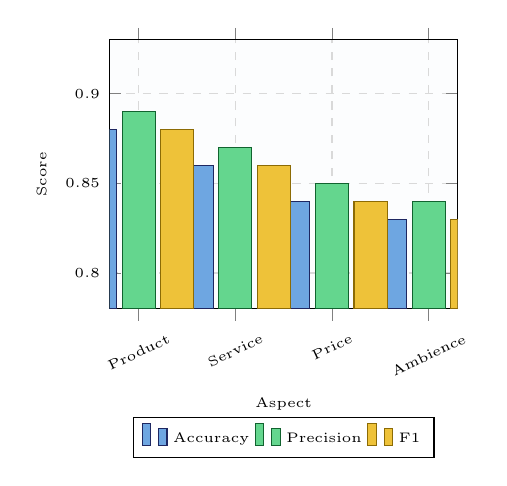
\begin{tikzpicture}
        \begin{axis}[
          ybar, bar width=0.42cm,
          width=6cm, height=5cm,
          xlabel={\tiny Aspect},
          ylabel={\tiny Score},
          symbolic x coords={Product,Service,Price,Ambience},
          xtick=data,
          xticklabel style={font=\tiny, rotate=25},
          ymin=0.78, ymax=0.93,
          ytick={0.80,0.85,0.90},
          yticklabel style={font=\tiny},
          legend style={font=\tiny, at={(0.5,-0.40)},
                        anchor=north, legend columns=3},
          grid=major, grid style={dashed,gray!30},
          axis background/.style={fill=lightgray!30}
        ]
          \addplot[fill=accentblue!80, draw=navyblue]
            coordinates {(Product,0.88)(Service,0.86)(Price,0.84)(Ambience,0.83)};
          \addplot[fill=posgreen!70, draw=posgreen!50!black]
            coordinates {(Product,0.89)(Service,0.87)(Price,0.85)(Ambience,0.84)};
          \addplot[fill=neuyellow!80, draw=neuyellow!60!black]
            coordinates {(Product,0.88)(Service,0.86)(Price,0.84)(Ambience,0.83)};
          \legend{Accuracy,Precision,F1}
        \end{axis}
      \end{tikzpicture}
      \end{center}
    \column{0.53\textwidth}
      \textbf{\color{navyblue}Confusion Matrix --- Service Aspect}
      \vspace{0.15cm}
      \small
      \begin{center}
      \begin{tabular}{lccc}
        \toprule
        & \textbf{Pred +} & \textbf{Pred 0} & \textbf{Pred $-$} \\
        \midrule
        \rowcolor{posgreen!15}
        \textbf{True +}   & \textbf{152} & 12 & 3 \\
        \textbf{True 0}   & 9  & \textbf{98}  & 7 \\
        \rowcolor{negred!10}
        \textbf{True $-$} & 2  & 8  & \textbf{134} \\
        \bottomrule
      \end{tabular}
      \end{center}
      \vspace{0.25cm}
      \textbf{\color{navyblue}Key Findings:}
      \begin{itemize}
        \item Macro-avg F1 = \textbf{0.85} across all aspects
        \item Neutral class hardest ($\approx 0.65$ confidence) due to ambiguity
        \item XAI correctly identified primary opinion word in \textbf{79--82\%}
        \item Health Score Pearson $r = 0.83$ vs.\ real-world ground truth
      \end{itemize}
  \end{columns}
\end{frame}

% ── SLIDE 13: THROUGHPUT BENCHMARKS ──────────────────────────
\begin{frame}{Performance Benchmarks \& Throughput}
  \begin{columns}[T]
    \column{0.5\textwidth}
      \textbf{\color{navyblue}Inference Throughput Comparison}
      \vspace{0.2cm}
      \begin{center}
      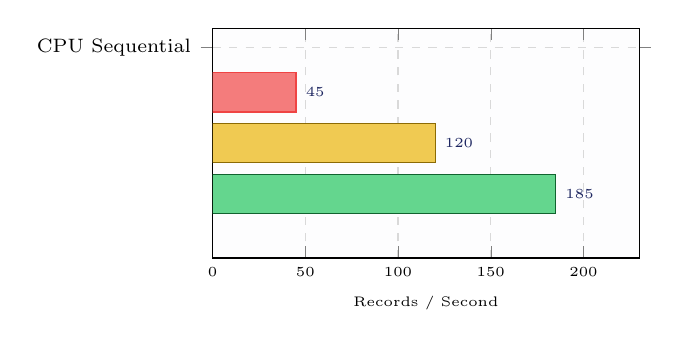
\begin{tikzpicture}
        \begin{axis}[
          xbar, bar width=0.5cm,
          width=7cm, height=4.5cm,
          xlabel={\tiny Records / Second},
          symbolic y coords={{GPU Batch-32},{CPU Batch-32},{CPU Sequential}},
          ytick=data,
          yticklabel style={font=\scriptsize},
          xmin=0, xmax=230,
          xticklabel style={font=\tiny},
          nodes near coords,
          nodes near coords style={font=\tiny\bfseries, color=navyblue},
          grid=major, grid style={dashed,gray!30},
          axis background/.style={fill=lightgray!20}
        ]
          \addplot[fill=negred!70, draw=negred]
            coordinates {(45,{CPU Sequential})};
          \addplot[fill=neuyellow!70, draw=neuyellow!60!black]
            coordinates {(120,{CPU Batch-32})};
          \addplot[fill=posgreen!70, draw=posgreen!50!black]
            coordinates {(185,{GPU Batch-32})};
        \end{axis}
      \end{tikzpicture}
      \end{center}
      \begin{center}
        \small\textbf{\color{posgreen}16--33$\times$ speedup} from batch processing
      \end{center}
    \column{0.48\textwidth}
      \textbf{\color{navyblue}Operation Benchmarks}
      \vspace{0.1cm}
      \small
      \rowcolors{2}{iceblue!20}{white}
      \begin{tabular}{>{\scriptsize}p{3.0cm} >{\scriptsize\bfseries}c >{\scriptsize\bfseries}c}
        \toprule
        \rowcolor{navyblue}\scriptsize\color{white}Operation &
        \color{white}CPU & \color{white}GPU \\
        \midrule
        BERT single inference & 500ms       & 30ms \\
        BERT batch-32         & 200ms/batch & 50ms/batch \\
        Zero-shot per review  & 300ms       & 80ms \\
        LOO attribution (10w) & 5s          & 1s \\
        500-review bulk run   & $\sim$3 min & $\sim$45s \\
        \bottomrule
      \end{tabular}
      \vspace{0.3cm}
      \begin{tcolorbox}[colback=navyblue!8, colframe=navyblue, arc=4pt]
        \small\textbf{\color{navyblue}Social Media Monitor Sources}\\[3pt]
        \scriptsize
        \faSatelliteDish\ Twitter/X API v2 (Bearer Token)\\
        \faPlay\ Google Play Scraper (no auth)\\
        \faPaste\ Manual Paste (fully offline)\\
        \faPlay\ Simulation Mode (CSV replay)
      \end{tcolorbox}
  \end{columns}
\end{frame}

% ── SLIDE 14: ADVANTAGES, LIMITATIONS & FUTURE ───────────────
\begin{frame}{Advantages, Limitations \& Future Scope}
  \begin{columns}[T]
    \column{0.33\textwidth}
      \begin{tcolorbox}[colback=posgreen!10, colframe=posgreen!60!black, arc=5pt,
                        title={\small\bfseries\faThumbsUp\ Key Advantages},
                        fonttitle=\color{white}, colbacktitle=posgreen!60!black]
        \scriptsize
        \faCheckCircle\ End-to-end BI pipeline\\[3pt]
        \faCheckCircle\ Explainability by design (4-layer XAI)\\[3pt]
        \faCheckCircle\ Zero-shot --- no labeled aspect data\\[3pt]
        \faCheckCircle\ Proactive churn intelligence (AUC 0.87)\\[3pt]
        \faCheckCircle\ Offline-first core (BERT, XAI, PDF)\\[3pt]
        \faCheckCircle\ bcrypt auth + MD5 deduplication
      \end{tcolorbox}
    \column{0.33\textwidth}
      \begin{tcolorbox}[colback=negred!10, colframe=negred, arc=5pt,
                        title={\small\bfseries\faExclamationTriangle\ Limitations},
                        fonttitle=\color{white}, colbacktitle=negred]
        \scriptsize
        \faTimes\ LOO: N BERT passes, slow on CPU\\[3pt]
        \faTimes\ SQLite write-locking limits concurrency\\[3pt]
        \faTimes\ Internet-dependent: Twitter, Groq, Translate\\[3pt]
        \faTimes\ Zero-shot adds 200--400ms per review\\[3pt]
        \faTimes\ Domain sensitivity for specialized vocabulary
      \end{tcolorbox}
    \column{0.33\textwidth}
      \begin{tcolorbox}[colback=accentblue!10, colframe=accentblue, arc=5pt,
                        title={\small\bfseries\faRocket\ Future Scope},
                        fonttitle=\color{white}, colbacktitle=accentblue]
        \scriptsize
        \faCloud\ Docker + Kubernetes on AWS/GCP\\[3pt]
        \faBolt\ Apache Kafka streaming pipeline\\[3pt]
        \faSync\ Continuous BERT fine-tuning (LoRA)\\[3pt]
        \faGlobe\ XLM-RoBERTa multilingual ABSA\\[3pt]
        \faMicrophone\ OpenAI Whisper ASR integration\\[3pt]
        \faMobileAlt\ React Native mobile application\\[3pt]
        \faLink\ Salesforce/HubSpot CRM webhooks
      \end{tcolorbox}
  \end{columns}
\end{frame}

% ── SLIDE 15: CONCLUSION ─────────────────────────────────────
{
\setbeamertemplate{footline}{}
\begin{frame}
  \begin{tikzpicture}[remember picture, overlay]
    \fill[navyblue] (current page.north west) rectangle (current page.south east);
    \fill[accentblue!25] (current page.north west) ++(2,-2)  circle (2.5cm);
    \fill[iceblue!15]    (current page.south east) ++(-2,2)  circle (3cm);
  \end{tikzpicture}
  \begin{center}
    {\color{iceblue}\Large\faChartBar}\\[0.2cm]
    {\color{white}\LARGE\textbf{Conclusion}}\\[0.4cm]
    \begin{tcolorbox}[colback=white!12, colframe=iceblue, arc=6pt, boxrule=1pt,
                      width=0.90\textwidth]
      \color{white}\small
      \textbf{BizDecisions AI} unifies five advanced AI capabilities ---
      BERT ABSA, XAI (LOO SHAP), Random Forest churn prediction, Groq LLM
      strategy generation, and zero-shot aspect detection --- into a single
      production-grade SaaS application accessible to non-technical users.
    \end{tcolorbox}
    \vspace{0.3cm}
    \begin{columns}[c]
      \column{0.25\textwidth}
        \begin{center}
          {\color{posgreen}\huge\textbf{0.85}}\\
          {\color{iceblue!80}\scriptsize Macro-avg F1}
        \end{center}
      \column{0.25\textwidth}
        \begin{center}
          {\color{neuyellow}\huge\textbf{33$\times$}}\\
          {\color{iceblue!80}\scriptsize Batch Speedup}
        \end{center}
      \column{0.25\textwidth}
        \begin{center}
          {\color{highlightblue}\huge\textbf{0.83}}\\
          {\color{iceblue!80}\scriptsize Health Score $r$}
        \end{center}
      \column{0.25\textwidth}
        \begin{center}
          {\color{negred!80}\huge\textbf{0.87}}\\
          {\color{iceblue!80}\scriptsize Churn AUC-ROC}
        \end{center}
    \end{columns}
    \vspace{0.4cm}
    \begin{tcolorbox}[colback=white!10, colframe=accentblue!60, arc=6pt, boxrule=0.8pt,
                      width=0.85\textwidth, halign=center]
      \color{iceblue}\small\itshape
      ``The technical gap between raw customer feedback and strategic business\\
       action can be bridged entirely through accessible AI.''
    \end{tcolorbox}
    \vspace{0.25cm}
    {\color{iceblue!80}\small\textbf{Sundara Thamizhan}
      $\cdot$ CB.PS.I5DAS22055 $\cdot$ April 2026}\\
    {\color{iceblue!60}\scriptsize Amrita Vishwa Vidyapeetham, Coimbatore}
  \end{center}
\end{frame}
}

\end{document}
